% report.tex
% Scientific article template in English
% Recommended compilation: pdflatex report.tex -> biber report -> pdflatex report.tex (x2)

\documentclass[11pt,a4paper]{report}

% Encoding and language
\usepackage[T1]{fontenc}
\usepackage[utf8]{inputenc}
\usepackage[english]{babel}

% Page layout
\usepackage{geometry}
\geometry{margin=2.5cm}
\usepackage{microtype}
\usepackage{placeins}
% Graphics, tables, mathematics
\usepackage{graphicx}
\usepackage{booktabs}
\usepackage{amsmath,amssymb,amsthm}
\usepackage{empheq}
\usepackage{siunitx}

% For floating algorithms with caption
\usepackage{algorithm}
%\usepackage{algorithmic}


\usepackage{algpseudocode}  % alternative to algorithmic, works with algorithm

% Links, citations
\usepackage[colorlinks=true,linkcolor=blue,citecolor=blue,urlcolor=blue]{hyperref}
\usepackage{csquotes}
% biblatex is loaded later with the desired options to avoid an "Option clash for package biblatex" error
\usepackage{minitoc}

\usepackage[
    backend=biber,
    style=numeric,   % <-- citations sous forme d'entiers
    sorting=none     % pour garder l'ordre d'apparition si tu veux
]{biblatex}

\addbibresource{biblio.bib}

% Useful environments
\theoremstyle{plain}
\newtheorem{theorem}{Theorem}[section]
\theoremstyle{definition}
\newtheorem{definition}{Definition}[section]

% Handy commands
\newcommand{\ie}{\textit{i.e.}}
\newcommand{\eg}{\textit{e.g.}}

% PDF metadata
\hypersetup{
    pdftitle={Automated Calibration of Physical Models for Musical Instruments},
    pdfauthor={Rodolphe Milton VIVANT},
    pdffitwindow=true
}

\title{Automated Calibration of Physical Models for Musical Instruments\\[0.5em]}

\author{Rodolphe Milton VIVANT\thanks{UFR de Mathématique et Informatique de Strasbourg, rodolphe.vivant3@etu-unistra.fr}}
\date{\today}

\begin{document}
\dominitoc
\maketitle

\begin{abstract}
This project focuses on the automated calibration of physical models for reed musical instruments. 
We develop a numerical framework to simulate wave propagation inside instruments with variable cross-sectional areas using the Discontinuous Galerkin Method (DGM). 
Special attention is given to the implementation of boundary conditions that model radiation and reed dynamics. 
The framework is validated against analytical solutions for uniform cross-sections and extended to non-uniform geometries, such as exponential and conical profiles. 
Results demonstrate accurate wave propagation, proper handling of complex boundaries, and convergence consistent with theoretical expectations. 
The proposed approach provides a foundation for efficient parameter calibration in virtual instrument models.



\vspace{3em}
Ce projet porte sur la calibration automatique de modèles physiques pour les instruments de musique à anche. 
Nous développons un cadre numérique pour simuler la propagation des ondes à l'intérieur d'instruments présentant des sections transversales variables, en utilisant la méthode de Galerkin discontinu (DGM). 
Une attention particulière est portée à la mise en œuvre des conditions aux limites modélisant la radiation et la dynamique de l'anche. 
Le cadre est validé par rapport à des solutions analytiques pour des sections uniformes et étendu à des géométries non uniformes, telles que les profils exponentiels et coniques. 
Les résultats montrent une propagation des ondes précise, une gestion correcte des conditions aux limites complexes et une convergence conforme aux prédictions théoriques. 
Cette approche fournit une base solide pour la calibration efficace des paramètres dans les modèles d'instruments virtuels.
\end{abstract}

\newpage
\setcounter{tocdepth}{2}
\tableofcontents

\newpage
\chapter{Introduction}

During my project of the thrid semester of the CSMI Master degree, I worked on the automated calibration 
of physical models for musical instruments. 
The goal of this project was to develop a method to automatically adjust the parameters of physical models 
so that they accurately reproduce the characteristic sounds of reed instruments. \newline
I worked under the supervision of Dr Emmanuel Franck, Dr Laurent Navoret and Dr Victor Michel-Dansac from 
the Institut de Recherche Mathématique Avancée (IRMA) in Strasbourg and Dr Juliette Chabassier from Modartt. \newline
Modartt (MOdels and Data for ARTs and Technology)\cite{Modartt} is a french company specialized in the development of artistic and technological application softwares.
In 2006, they released \textit{Pianoteq}, a software that simulates the sound of various musical instruments using physical modeling techniques isntead 
of relying on pre-recorded samples. \newline
First, we present the context of reed instruments and the state of the art of the mathematical modeling of the wave equation inside these instruments.
Then, we describe the numerical methods used to solve the wave equation with different types of cross-sectional 
area (uniform, exponential, conical) using the Discontinuous Galerkin Method (DGM). We will particularly focus on the implementation of the boundary conditions
that represent a crucial aspect of the behavior of the sound produced by the instrument.
Finally, we present the results of the numerical simulations and the performance analysis of the implemented method.

\minitoc

\newpage
\section{Reed Instruments}
A reed is a thin, flexible lamina mounted at the mouthpiece or at the entrance of an air column resonator that acts \cite{Universalis_Anche} \cite{chaigne:hal-05370840} as a valve that controls the airflow driven by a pressure difference between the upstream region 
(the player’s mouth) and the downstream region (the mouthpiece or mouthpiece tip of the instrument). \newline
There are two principal categories of reed instruments:
\begin{itemize}
    \item Free reeds (harmonicas, accordions, ...).
    \item Beating reeds (clarinets, saxophones, ...).
\end{itemize}
% Figure : schéma de l'anche / embouchure
\begin{figure}[htbp]
    \centering
    % Remplacez 'figs/reed.png' par le chemin et l'extension réels de votre image (pdf, png, jpg...)
    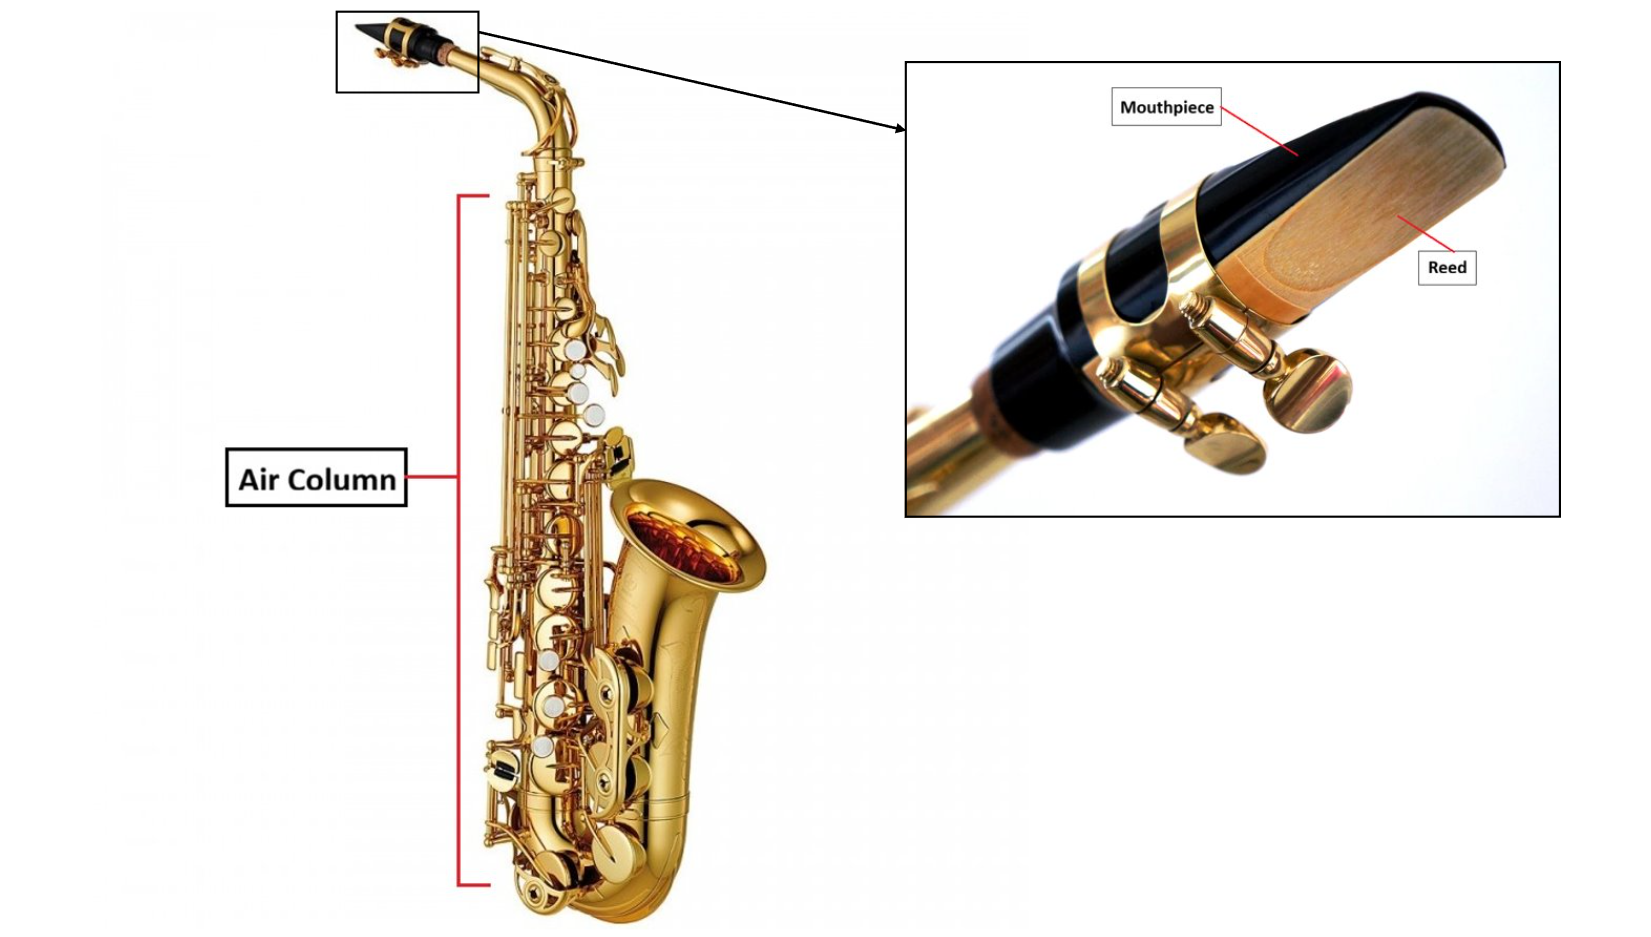
\includegraphics[width=0.75\textwidth]{Images/reed_column.png}
    \caption{Reed and saxophone.}
    \label{fig:reed_schematic}
\end{figure}


\section{State of the art}
The equations governing the behavior of reed instruments are mathematically described \cite{MAMAMIA2024} by a set of coupled 
differential equations (Partial Differential Equations - PDEs, Ordinary Differential Equations - ODEs, and 
algebraic equations). These equations capture the complex interactions between the pressure ($p$), the acoustic
volume velocity ($v$) \eqref{eq:1a} \eqref{eq:1b}, radiative phenomenons happening at the bell of the instrument($\phi$) \eqref{eq:1c} \eqref{eq:1d}, 
and the effects of the instrumental player \eqref{eq:1e} \eqref{eq:1f} :

% Système d'équations décrivant un modèle réducteur pour un instrument à anche
\begin{subequations}
\begin{empheq}[left=\empheqlbrace]{align}
  \frac{S(x)}{c S^\ast}\,\partial_t p(x,t) + \partial_x v(x,t) &= 0 \label{eq:1a}\\[4pt]
  \frac{S^\ast}{c S(x)}\,\partial_t v(x,t) + \partial_x p(x,t) &= 0 \label{eq:1b}\\[4pt]
  Z^\ast_T\,\partial_t \phi + \sqrt{\alpha}\,p(L,t) &= 0 \label{eq:1c}\\[4pt]
  -\frac{\beta}{Z^\ast_T}\,p(L,t) + v(L,t) + \sqrt{\alpha}\,\phi &= 0 \label{eq:1d}\\[4pt]
  -v(0,t) + \zeta \ell(y)\,F(\gamma - p(0,t)) + \varepsilon\frac{\kappa}{\omega_r}\,\partial_t y &= 0 \label{eq:1e}\\[6pt]
  \frac{1}{\omega_r^2}\,\partial_{tt} y + \frac{1}{Q_r\omega_r}\,\partial_t y + y - 1 
  &= \varepsilon(\gamma - p(0,t)) \label{eq:1f}
\end{empheq}
\end{subequations}

where $S(x)$ is the cross-sectional area of the instrument at position $x$, $S^\ast$ is a reference area,
$c$ is the speed of sound, $Z^\ast_T$ is a reference acoustic impedance, 
$\alpha$ and $\beta$ are parameters related to the radiation effects, $L$ is the length of the instrument,
$\zeta_\ell(y)$ is a function representing the lip-reed coupling, $F$ is a nonlinear function ($F(\Delta p)=\Delta p \, \text{sign} (\Delta p)$),
$\gamma$ is the dimensionless blowing pressure, $\varepsilon$ =-1 for a reed instrument, 
$\kappa$ is a parameter related to the lip dynamics, $\omega_r$ is the reed's (or lips') frequency ($=2\pi f_r$), 
$Q_r$ is the quality factor of the reed, and $y$ is the dimensionless reed opening. \newline
This kind of system of equation can already be solved numerically with Openwind \cite{OpenwindInria}.

\section{Objectives}
The main objectives of this project are: \\
In JAX framework:
\begin{enumerate}
    \item Implement a discontinous Galerkin discretization of the mixed form of the wave equation and numerically solve it.
    \item Implement the Left Hand Side boundary conditions (equations \eqref{eq:1c} and \eqref{eq:1d}) coupled with the DG solver.
    \item Implement the Right Hand Side boundary conditions (equations \eqref{eq:1e} and \eqref{eq:1f}) coupled with the DG solver.
    \item Compute the gradient with respect to all the problem parameters.   
\end{enumerate}

\newpage
\chapter{Methods}
\minitoc
\vspace{1em}
In this section, we present the numerical methods used to solve the wave equation with variable cross-sectional area
using the Discontinuous Galerkin Method (DGM) and the analytical solution in the simple case of a constant cross-sectional area.
We will fist introduce the DGM, then we will present its application to our specific problem described in Section 1.2 with 
the explicit expression of the numerical fluxes and the boundary conditions.
Finally, we will derive the analytical solution for the case of a constant cross-sectional area.

\newpage
\section{Discontinuous Galerkin Method \cite{HesthavenWarburton2008}}
The Discontinuous Galerkin Method (DGM) is a numerical technique used to solve partial differential equations (PDEs). 
Let's consider an equation of the form :
\begin{equation}
    \frac{\partial u}{\partial t} + \frac{\partial F(u)}{\partial x} = 0,
\end{equation}
where $u(x,t)$ is the unknown function and $F(u)$ is a flux function. \newline
The DGM involves the following steps:
\begin{enumerate}
    \item \textbf{Domain Discretization:} Divide the spatial domain into a finite number of elements or cells.
    \item \textbf{Basis Functions:} Choose a set of basis functions (often polynomials) to represent the solution within each element.
    \item  \textbf{Weak Formulation:} Multiply the PDE by a test function (which can be one of the basis functions) and integrate over each element to obtain the weak form of the equation.
    \item \textbf{Numerical Fluxes:} Define numerical fluxes at the interfaces between elements to ensure stability and consistency.
    \item \textbf{Time Integration:} Use an appropriate time-stepping method (e.g., Runge-Kutta;, Euler Explicit) to advance the solution in time.
\end{enumerate} 

\section{Time discretization and weak formulation}

Let $u^n(x)$ denote the numerical approximation of the solution at time $t^n$.
A first-order explicit time discretization yields
\begin{equation}
u^{n+1}(x) = u^n(x) - \Delta t \, \partial_x F\big(u^n(x)\big).
\label{eq:time_disc}
\end{equation}

Let $\varphi_i(x)$ be a test function. The weak formulation on a single cell
$\Omega_k$ reads
\begin{equation}
\int_{\Omega_k} \varphi_i(x) u^{n+1}(x)\, dx
=
\int_{\Omega_k} \varphi_i(x) u^n(x)\, dx
-
\Delta t \int_{\Omega_k} \varphi_i(x) \partial_x F\big(u^n(x)\big)\, dx.
\label{eq:weak_form_1}
\end{equation}

Applying integration by parts to the second term gives
\begin{equation}
\int_{\Omega_k} \varphi_i(x) u^{n+1}(x)\, dx
=
\int_{\Omega_k} \varphi_i(x) u^n(x)\, dx
+
\Delta t \int_{\Omega_k} \partial_x \varphi_i(x) F\big(u^n(x)\big)\, dx
-
\Delta t \left[ \varphi_i(x) F\big(u^n(x)\big) \right]_{\partial \Omega_k}.
\label{eq:weak_form_2}
\end{equation}

The boundary term is approximated using a numerical flux.
Expanding the solution in the local basis $\{\varphi_j\}$,
\begin{equation}
u^{n+1}(x)\big|_{\Omega_k} = \sum_j \alpha^{n+1}_{k,j} \varphi_j(x),
\end{equation}
leads to the local system
\begin{equation}
\sum_j \alpha^{n+1}_{k,j}
\int_{\Omega_k} \varphi_i(x)\varphi_j(x)\, dx
=
\int_{\Omega_k} \varphi_i(x) u^n(x)\, dx
+
\Delta t \int_{\Omega_k} \partial_x \varphi_i(x) F\big(u^n(x)\big)\, dx
-
\Delta t \left[ \varphi_i(x) F\big(u^n(x)\big) \right]_{\partial \Omega_k}.
\label{eq:dg_local}
\end{equation}

Defining the local mass matrix
\begin{equation}
M_{ij} = \int_{\Omega_k} \varphi_i(x)\varphi_j(x)\, dx,
\end{equation}
the update can be written compactly as
\begin{equation}
M \, \boldsymbol{\alpha}^{n+1}_k = \mathbf{b}_k,
\label{eq:matrix_form}
\end{equation}
where $\mathbf{b}_k$ contains the volume and numerical flux contributions.

\section{Discontinuous Galerkin method in our context}

\subsection{Conservative form}

We consider the mixed formulation of the one-dimensional wave equation.
Introducing the vector of unknowns
\begin{equation}
\mathbf{u} =
\begin{pmatrix}
p \\
v
\end{pmatrix},
\end{equation}
the system can be written in conservative form as
\begin{equation}
C(x)\, \partial_t \mathbf{u} + \partial_x \big( A \mathbf{u} \big) = 0,
\label{eq:conservative_form}
\end{equation}
with
\begin{equation}
C(x) =
\begin{pmatrix}
\dfrac{S(x)}{c S^*} & 0 \\
0 & \dfrac{S^*}{c S(x)}
\end{pmatrix},
\qquad
A =
\begin{pmatrix}
0 & 1 \\
1 & 0
\end{pmatrix}.
\end{equation}

The initial conditions are given by
\begin{equation}
p(x,0) = p_0(x), \qquad v(x,0) = v_0(x).
\end{equation}

\subsection{Mesh and DG space}

Let
\begin{equation}
0 = x_0 < x_1 < \dots < x_N = L,
\qquad
K_j = (x_{j-1}, x_j), \quad j = 1,\dots,N.
\end{equation}

We seek an approximate solution
\begin{equation}
\mathbf{u}_h = (p_h, v_h)^T \in (V_h^k)^2,
\end{equation}
where
\begin{equation}
V_h^k =
\left\{
u \in L^2(0,L) \;\middle|\;
u|_{K_j} \in \mathbb{P}_1(K_j)
\right\}.
\end{equation}

\subsection{Local DG formulation}

For each element $K_j$ and for each test function vector
\begin{equation}
\boldsymbol{\Phi} = (\varphi_p, \varphi_v)^T \in (\mathbb{P}_1(K_j))^2,
\end{equation}
the local weak formulation reads
\begin{equation}
\int_{K_j} C(x)\, \partial_t \mathbf{u}_h \cdot \boldsymbol{\Phi}\, dx
-
\int_{K_j} A \mathbf{u}_h \cdot \partial_x \boldsymbol{\Phi}\, dx
+
\widehat{\mathbf{F}}_{j+\frac12} \cdot \boldsymbol{\Phi}(x_j^-)
-
\widehat{\mathbf{F}}_{j-\frac12} \cdot \boldsymbol{\Phi}(x_{j-1}^+)
= 0.
\label{eq:dg_local_vector}
\end{equation}

The physical flux is defined as
\begin{equation}
\mathbf{F}(\mathbf{u}) = A \mathbf{u}
=
\begin{pmatrix}
v \\
p
\end{pmatrix}.
\end{equation}

\subsection{Rusanov flux}

At each interface $x_{j+\frac12}$, the Rusanov (local Lax--Friedrichs) flux is defined by
\begin{equation}
\widehat{\mathbf{F}} =
\frac{1}{2}
\left(
\mathbf{F}(\mathbf{u}^-) + \mathbf{F}(\mathbf{u}^+)
\right)
-
\frac{\lambda_{j+\frac12}}{2}
\left(
\mathbf{u}^+ - \mathbf{u}^-
\right),
\label{eq:rusanov}
\end{equation}
where $\lambda_{j+\frac12}$ denotes the maximum characteristic speed at the interface.
At that state of development, the 


\subsection{Explicit flux}
By denoting
$$
\mathbf U^\pm =
\begin{pmatrix}
p^\pm\\
v^\pm
\end{pmatrix},
\qquad
\mathbf F(\mathbf U)=
\begin{pmatrix}
v\\
p
\end{pmatrix},
$$
The numerical flux at each interface is given by :
$$
\widehat{\mathbf F} =
\begin{pmatrix}
\widehat{v}\\
\widehat{p}
\end{pmatrix},
$$
with
$$
\boxed{
\begin{aligned}
\widehat{v}
& =
\frac12\left(v^-+v^+\right)
-
\frac{c}{2}\left(p^+-p^-\right),
\\
\widehat{p}
& =
\frac12\left(p^-+p^+\right)
-
\frac{c}{2}\left(v^+-v^-\right).
\end{aligned}
}
$$

\subsection{Final DG formulation}
For each element $K_j=(x_{j-1},x_j)$ and 
for each test function $w_p,w_v\in\mathbb P^k(K_j)$, 
the DG formulation of the mixed form of the wave equation reads :

\begin{equation}
\begin{aligned}
\int_{K_j} \frac{S(x)}{cS^\ast}\,
\partial_t p_h \, \phi_p \, dx
&-
\int_{K_j} v_h \, \partial_x \phi_p \, dx \\
&+
\widehat{v}_{j+\frac12}\, \phi_p(x_j^-)
-
\widehat{v}_{j-\frac12}\, \phi_p(x_{j-1}^+)
=0,
\end{aligned}
\label{eq:dg_wave_p}
\end{equation}

\begin{equation}
\begin{aligned}
\int_{K_j} \frac{S^\ast}{cS(x)}\,
\partial_t v_h \, \phi_v \, dx
&-
\int_{K_j} p_h \, \partial_x \phi_v \, dx \\
&+
\widehat{p}_{j+\frac12}\, \phi_v(x_j^-)
-
\widehat{p}_{j-\frac12}\, \phi_v(x_{j-1}^+)
=0.
\end{aligned}
\label{eq:dg_wave_v}
\end{equation}
All the dependence on the variable cross-sectional area $S(x)$ is contained in the mass matrix C(x). 
This property ensures a uniform wave speed c and a CFL condition independent of S(x)

\subsection{Boundary conditions}

One of the difficulties when simulating wave propagation in a wind instrument is to correctly
compute the influence of the exterior environment at the open end of the instrument. \cite{thibault}
To do so, we use a condition of radiation impedance. 
On the right-hand boundary ($x = L$), the acoustic field is coupled to a boundary dynamical system.
The boundary conditions are derived from equations~(1c)--(1d).

The boundary model reads:
\begin{equation}
\begin{cases}
Z^\ast_T\,\partial_t \phi(t)
+ \sqrt{\alpha}\, p(L,t) = 0,
\\[0.4em]
-\dfrac{\beta}{Z^\ast_T}\, p(L,t)
+ v(L,t)
+ \sqrt{\alpha}\,\phi(t) = 0.
\end{cases}
\label{eq:bc_ode_pde}
\end{equation}

The first equation governs the time evolution of the boundary variable $\phi(t)$, while the second
equation provides a dynamic impedance relation between pressure and velocity at the boundary.
\begin{equation}
v(L,t) = \frac{\beta}{Z^\ast_T} p(L,t) - \sqrt{\alpha}\,\phi(t).
\tag{BC}
\end{equation}

From the characteristic variables defined as :
\begin{equation}
w^+ = p + v,
\qquad
w^- = p - v.
\end{equation}

At the right boundary, the wave $\omega^+$ is outgoing while $\omega^-$ is incoming.
The boundary condition must therefore provide a relation to determine $w^-$.

From the definition of $w^-$ and the boundary condition (BC), we have:
\begin{equation}
    \begin{aligned}
        w^-
        &= p - v \\
        &= p - \left( \frac{\beta}{Z^\ast_T} p - \sqrt{\alpha}\,\phi \right) \\
        &= \left(1 - \frac{\beta}{Z^\ast_T}\right)p + \sqrt{\alpha}\,\phi.
    \end{aligned}
\end{equation}

And the expression of $p$ in terms of $w^+$ and $w
^-$ is :
\begin{equation}
p = \frac{w^+ + w^-}{2}.
\end{equation}

By substituting this into the previous equation, we obtain:
\begin{equation}
w^-
= \left(1 - \frac{\beta}{Z^\ast_T}\right)\frac{w^+ + w^-}{2} + \sqrt{\alpha} \phi.
\end{equation}

So the incoming wave $w^-$ can be expressed as:
\begin{equation}
\boxed{
w^- =
\frac{1 - \frac{\beta}{Z^\ast_T}}{1 + \frac{\beta}{Z^\ast_T}}
w^+
+
\frac{2\sqrt{\alpha}}{1 + \frac{\beta}{Z^\ast_T}} \phi
}
\label{eq:wminus_final}
\end{equation}

This expression is used to impose the boundary condition in the numerical flux of the DG scheme.
In the DG framework, boundary conditions are enforced weakly through the numerical flux.
At the right boundary, the outgoing characteristic is obtained from the interior solution,
while the incoming characteristic is prescribed by the boundary condition.
The relation~\eqref{eq:wminus_final} provides the value of the incoming wave $w^-$, from which
the boundary state is reconstructed and used as the exterior state in the numerical flux.
\\
Note : In practice, the boundary ODE~\eqref{eq:bc_ode_pde} is discretized in time using the same time
integration scheme as the DG solver, ensuring a consistent coupling between the PDE and ODE systems. (see Algorithm~\ref{alg:dg_scheme_boundary_ode_rk2}).

\section{Numerical Algorithm: DG Scheme with Boundary ODE}

The following algorithm implements the Discontinuous Galerkin (DG) scheme 
for the one-dimensional mixed wave equation with variable cross-section. 
The right boundary at $x=L$ is coupled to an auxiliary ODE to dynamically 
impose the boundary condition. The DG update can be performed using either 
the explicit Euler method or a second-order Runge-Kutta scheme.

\begin{algorithm}[H]
\caption{DG scheme with boundary ODE at right boundary ($x=L$)}
\begin{algorithmic}[1]
\State \textbf{Initialization:}
\State \quad Project $p_0(x), v_0(x)$ onto DG space
\State \quad Initialize $\phi^0$

\For{$n = 0, \dots, N_t-1$}

    \State \textbf{1. Compute boundary characteristics at $x=L$:}
    \[
        w^{+,n} = p_h^n(L^-) + v_h^n(L^-)
    \]

    \State \textbf{2. Incoming wave (boundary condition):}
    \[
        w^{-,n} = a\, w^{+,n} + b\, \phi^n,
    \quad
        a = \frac{1 - \beta/(Z^\ast_T)}{1 + \beta/(Z^\ast_T)},
    \quad
        b = \frac{2 \sqrt{\alpha}}{1 + \beta/(Z^\ast_T)}
    \]

    \State \textbf{3. Reconstruct ghost state:}
    \[
        p^{+,n} = \tfrac{1}{2}(w^{+,n} + w^{-,n}),
        \quad
        v^{+,n} = \tfrac{1}{2}(w^{+,n} - w^{-,n})
    \]

    \State \textbf{4. Compute numerical fluxes} $\hat{\mathbf F}^n$
    \State \textbf{5. DG residual:}
    \[
        k_1^u = \mathcal{L}(u^n,\phi^n)
    \]

    \State \textbf{6. Boundary ODE residual:}
    \[
        k_1^\phi = -\frac{\sqrt{\alpha}}{Z^\ast_T}\, p_h^n(L^-)
    \]

    \If{Euler time integration}

        \State \textbf{7a. Euler update:}
        \[
            u^{n+1} = u^n + \Delta t\, k_1^u,
            \quad
            \phi^{n+1} = \phi^n + \Delta t\, k_1^\phi
        \]

    \Else \Comment{RK2 mixed DG--ODE}

        \State \textbf{7b. Midpoint stage:}
        \[
            u^{n+\frac12} = u^n + \tfrac{\Delta t}{2} k_1^u,
            \quad
            \phi^{n+\frac12} = \phi^n + \tfrac{\Delta t}{2} k_1^\phi
        \]

        \State Recompute boundary characteristics using $u^{n+\frac12}$:
        \[
            w^{+,n+\frac12} = p_h^{n+\frac12}(L^-) + v_h^{n+\frac12}(L^-)
        \]

        \State Incoming wave at midpoint:
        \[
            w^{-,n+\frac12} = a\, w^{+,n+\frac12} + b\, \phi^{n+\frac12}
        \]

        \State Reconstruct midpoint ghost state and fluxes

        \State \textbf{8. Second-stage residuals:}
        \[
            k_2^u = \mathcal{L}(u^{n+\frac12},\phi^{n+\frac12}),
            \quad
            k_2^\phi = -\frac{\sqrt{\alpha}}{Z^\ast_T}\,
            p_h^{n+\frac12}(L^-)
        \]

        \State \textbf{9. RK2 update:}
        \[
            u^{n+1} = u^n + \Delta t\, k_2^u,
            \quad
            \phi^{n+1} = \phi^n + \Delta t\, k_2^\phi
        \]

    \EndIf

\EndFor
\end{algorithmic}
\label{alg:dg_scheme_boundary_ode_rk2}
\end{algorithm}



\section{Analytical Solution for Constant Section ($S(x)=S^\ast=1$)}

To assess the accuracy of the Discontinuous Galerkin (DG) implementation, we consider a uniform duct cross-section $S(x)=S^\ast=1$, for which an analytical solution is available. The governing equations read
\begin{align}
    \partial_t p + c\,\partial_x v &= 0, \\
    \partial_t v + c\,\partial_x p &= 0,
\end{align}
supplemented with the boundary conditions \eqref{eq:1c}--\eqref{eq:1d}.

\subsection{Riemann Invariants}

Introducing the characteristic variables
\begin{equation}
    w^+_{pde} := p+v, \qquad w^-_{pde} := p-v,
\end{equation}
the system decouples into two transport equations:
\begin{align}
    \partial_t w^+_{pde} + c\,\partial_x w^+_{pde} &= 0, \\
    \partial_t w^-_{pde} - c\,\partial_x w^-_{pde} &= 0.
\end{align}
With initial data $p(x,0)=p_0(x)$ and $v(x,0)=v_0(x)$, this yields
\begin{equation}
    w^+_{pde}(x,t) = w_0^+(x-ct), \qquad
    w^-_{pde}(x,t) = w_0^-(x+ct),
\end{equation}
where $w_0^\pm = p_0 \pm v_0$.
\subsection{Derivation of the Boundary Conditions in Characteristic Variables}

\subsubsection{Physical boundary conditions}

At the right boundary $x=L$, we consider an impedance-type termination described by an
auxiliary variable $\phi(t)$, governed by the following system (equations \eqref{eq:1c}--\eqref{eq:1d}):
\begin{align}
    Z_T^\ast \,\partial_t \phi(t) + \sqrt{\alpha}\, p(L,t) &= 0,
    \label{eq:bc_phi_phys}\\
    -\frac{\beta}{Z_T^\ast}\, p(L,t) + v(L,t) + \sqrt{\alpha}\,\phi(t) &= 0.
    \label{eq:bc_pv_phys}
\end{align}
This formulation models the dynamic response of the boundary.

\subsubsection{Characteristic variables}

Let's introduce again the Riemann (characteristic) variables
\begin{equation}
    w^+ = p + v, \qquad
    w^- = p - v,
\end{equation}
with inverse relations
\begin{equation}
    p = \frac12 (w^+ + w^-), \qquad
    v = \frac12 (w^+ - w^-).
\end{equation}

\subsubsection{Algebraic boundary condition}

Substituting the characteristic variables into \eqref{eq:bc_pv_phys} yields
\begin{align}
    -\frac{\beta}{Z_T^\ast}\,\frac{w^+ + w^-}{2}
    + \frac{w^+ - w^-}{2}
    + \sqrt{\alpha}\,\phi
    &= 0.
\end{align}
Multiplying by $2$ and rearranging terms gives
\begin{align}
    \left(-1 - \frac{\beta}{Z_T^\ast}\right) w^-
    + \left(1 - \frac{\beta}{Z_T^\ast}\right) w^+
    + 2\sqrt{\alpha}\,\phi
    &= 0,
\end{align}
which leads to the outgoing characteristic at the boundary:
\begin{equation}
    \boxed{
    w^-(L,t)
    =
    a\, w^+(L,t)
    + b\, \phi(t)
    }
    \label{eq:wminus_bc}
\end{equation}
with
\begin{equation}
    a = \frac{1-\beta/Z_T^\ast}{1+\beta/Z_T^\ast},
    \qquad
    b = \frac{2\sqrt{\alpha}}{1+\beta/Z_T^\ast}.
\end{equation}

\subsubsection{Dynamic equation for the auxiliary variable}

The dynamic boundary condition \eqref{eq:bc_phi_phys} can be rewritten as
\begin{equation}
    \partial_t \phi
    + \frac{\sqrt{\alpha}}{Z_T^\ast}\, p(L,t) = 0.
\end{equation}
Using $p = (w^+ + w^-)/2$ and substituting \eqref{eq:wminus_bc} for $w^-$, we obtain a closed
ordinary differential equation:
\begin{equation}
    \boxed{
    \partial_t \phi
    + c_1\, (1+a) \, w^+(L,t)
    + c_2\, \phi(t)
    = 0
    }
\end{equation}
where
\begin{equation}
    c_1 = \frac{\sqrt{\alpha}}{2 Z_T^\ast},
    \qquad
    c_2 = c_1\, b.
\end{equation}

\subsubsection{Definition of the reflected wave}

The free outgoing characteristic associated with the initial condition is
\begin{equation}
    w^-_{pde}(x,t) = w_0^-(x+ct).
\end{equation}
The boundary generates an additional reflected contribution, defined at $x=L$ by
\begin{equation}
    \boxed{
    w^-_{\mathrm{ref}}(L,t)
    :=
    a\, w^+_{pde}(L,t)
    + b\, \phi(t)
    }.
\end{equation}
This reflected wave is propagated into the domain along characteristics:
\begin{equation}
    w^-_{\mathrm{ref}}(x,t)
    =
    w^-_{\mathrm{ref}}
    \!\left(L,\, t - \frac{L-x}{c}\right),
    \qquad x \le L.
\end{equation}

The total outgoing characteristic is therefore
\begin{equation}
    w^-(x,t)
    =
    w^-_{pde}(x,t)
    + w^-_{\mathrm{ref}}(x,t).
\end{equation}

\subsubsection{Interpretation}

The impedance boundary condition acts as a dynamic reflection operator: the incoming
characteristic $w^+$ excites the auxiliary variable $\phi(t)$, which in turn generates
a reflected wave $w^-_{\mathrm{ref}}$ propagating back into the computational domain.

\subsection{Construction of the Analytical Solution}

The reflected characteristic $w^-_{ref}(L,t)$ is propagated into the domain along the characteristic lines with velocity $-c$. The total characteristics are therefore
\begin{align}
    w^+(x,t) &= w^+_{pde}(x,t) = w_0^+(x-ct), \\
    w^-(x,t) &= w^-_{pde}(x,t) + w^-_{ref}(x,t)
             = w_0^-(x+ct) + w^-_{ref}(x,t).
\end{align}
The pressure and velocity fields are finally reconstructed as
\begin{equation}
\begin{aligned}
    p(x,t) &= \tfrac12 \bigl[w^+(x,t) + w^-(x,t)\bigr], \\
    v(x,t) &= \tfrac12 \bigl[w^+(x,t) - w^-(x,t)\bigr].
\end{aligned}
\label{eq:exact_sol}
\end{equation}

This analytical solution is implemented in the function \texttt{exact\_solution\_characteristics} and serves as a reference to assess the accuracy of the DG scheme.



\chapter{Numerical Results}

\minitoc
\vspace{1em}
In this section, we present numerical results obtained using the Discontinuous Galerkin Method (DGM) 
for simulating wave propagation in a one-dimensional domain with variable cross-sectional area.
We will first describe the initial conditions and simulation parameters used in the experiments.
Then, we will present the results of the DGM solver for both uniform and non-uniform cross-sections(exponential and conical shapes),
with an analysis of the convergence of the method for the uniform cross-section case. 
Finally, we will present some performance benchmarks of the JAX implementation.

\newpage
\section{Initial Condition}
The initial pressure profile is defined as a smooth compactly supported bump function
centered at $x=L/2$. Introducing the rescaled variable
\begin{equation}
\xi(x) = \frac{4}{L}\left(x - \frac{L}{2}\right),
\end{equation}
the initial condition reads
\begin{equation}
p_0(x) =
\begin{cases}
\dfrac{\phi_0}{4}\,
\exp\!\left(1 - \dfrac{1}{1-\xi(x)^2}\right),
& \text{if } |\xi(x)| < 1, \\[1.2ex]
0, & \text{otherwise}.
\end{cases}
\end{equation}

The initial acoustic volume velocity is set to zero:
\begin{equation}
v_0(x) = 0.
\end{equation}

\section{Simulation Parameters}
Here are the parameters used in the simulations presented in this section.
We used the same set of parameters for all the test cases to ensure consistency 
and comparability of the results.
\begin{table}[h!]
\centering
\begin{tabular}{c cccccc}
\hline
Parameters & $\alpha$ & $\beta$ & $S^\ast$ & c & $Z^\ast_T$ & CLF \\
\hline
Values & 0.1 & 0.2 & 1 & 1 & 1.0 & 0.05 \\
\hline
\end{tabular}
\caption{Simulation parameters used in the DG P1 solver.}
\label{tab:sim_parameters}
\end{table}

These parameters define the physical properties of the wave propagation and take into
account certain aspects of the geometry of the instrument. 

\section{DG Method results}

\subsection{Uniform cross-section}

In the case of a uniform cross-section $S(x) = S^* = 1$, the analytical solution described in \eqref{eq:exact_sol} is available for validation.
In a future work, we might use the numerical solution obtained with Openwind as a reference for 
the comparaison when dealing with non-uniform cross-sections.

\subsubsection{Solution plots}

\begin{figure}[htbp]
    \centering
    % Remplacez 'figs/dg_solution.png' par le chemin et l'extension réels de votre image (pdf, png, jpg...)
    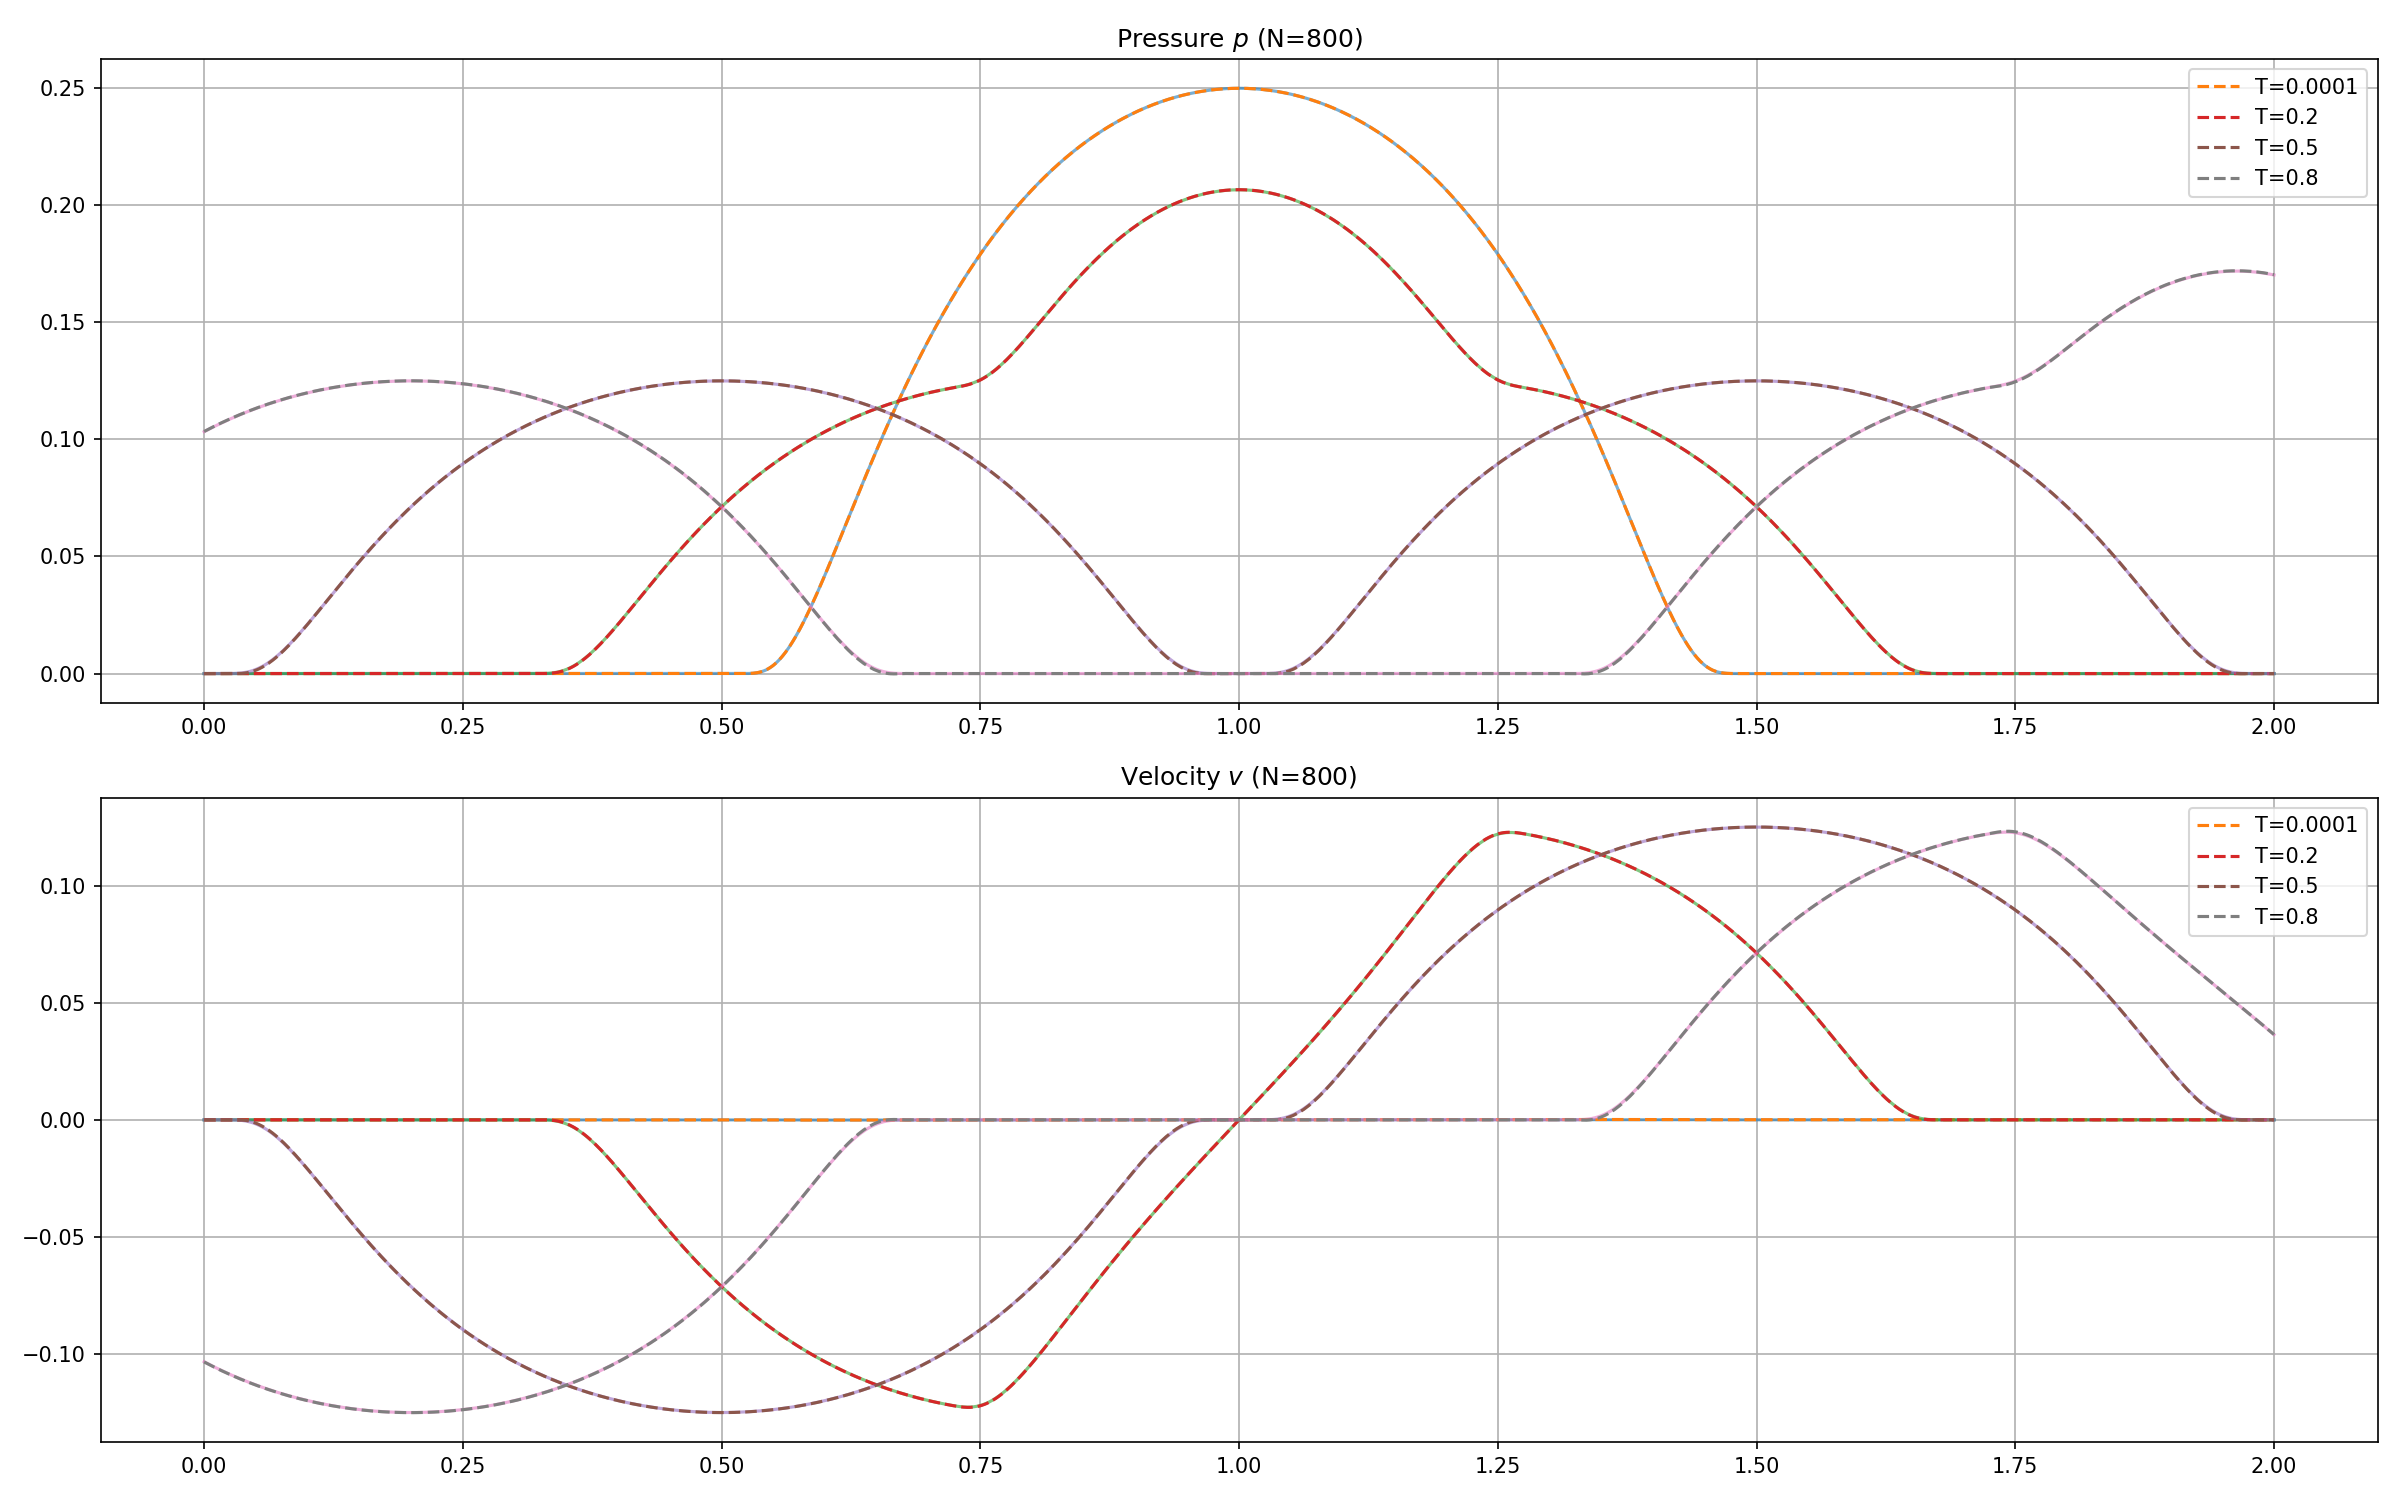
\includegraphics[width=0.9\textwidth]{Images/dg_solution_const_N800.png}
    \caption{DG numerical solutions constant cross-section.}
    \label{fig:dg_solution_const}
\end{figure}

As shown in Figure \ref{fig:dg_solution_const}, the numerical solution obtained using the Discontinuous Galerkin Method accurately captures 
the wave propagation over time described in \ref{eq:exact_sol}. The method effectively resolves the wave fronts 
and maintains stability throughout the simulation.
Inside the domain (Instrument), we can observe the proper propagation of the initial pressure bump, splitting into left-going and right-going waves for the pressure 
and velocity fields. At the right boundary, the interaction with the radiation condition seems to be correctly
computed hence demonstrating the method's capability to handle complex boundary conditions.

\FloatBarrier 
\subsubsection{Convergence study}
The convergence of the DG method is verified by comparing the numerical solution to the analytical solution at various size of discretisation with an Explicit Euler
time integration scheme and a Runge-Kutta 2nd order scheme by computing the $L^2$ norm of the error at final time $T=0.5\ \mathrm{s}$ and $T=0.8\ \mathrm{s}$ using 
the $L^2$ error.
This two final times are chosen to observe the solution before and after the wave has interacted with the right boundary to see the effect of the boundary condition on the convergence.


\begin{figure}[htbp]
    \centering
    \begin{minipage}[t]{0.48\textwidth}
        \centering
        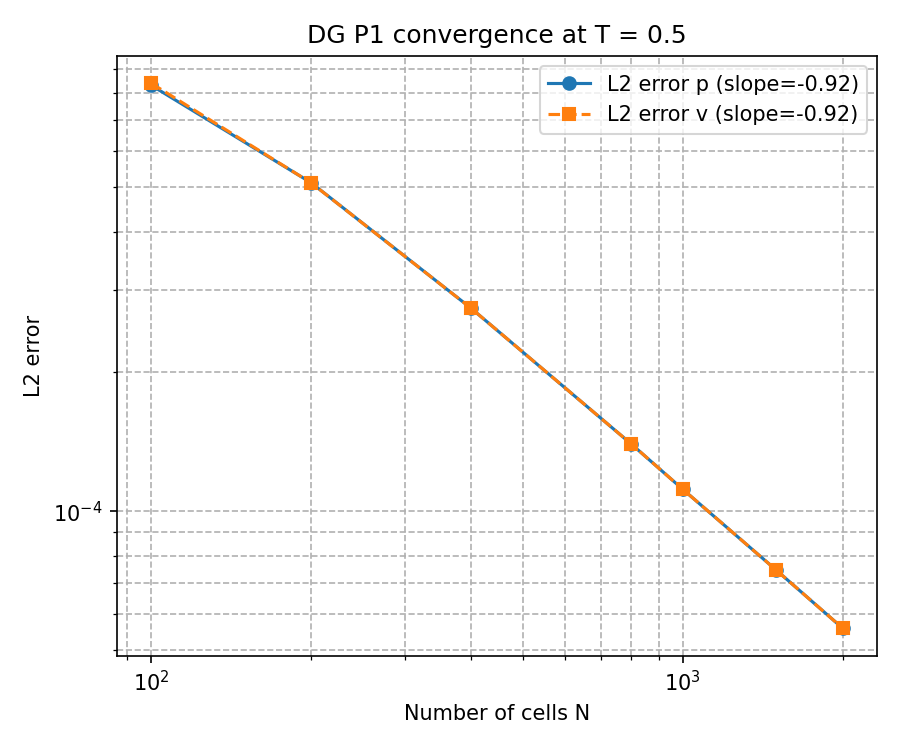
\includegraphics[width=\textwidth]{Images/dg_convergence_T0.5_euler.png}
        \caption{Convergence of the DG method with Explicit Euler scheme.}
        \label{fig:convergence_plot_euler_t_05}
    \end{minipage}
    \hfill
    \begin{minipage}[t]{0.48\textwidth}
        \centering
        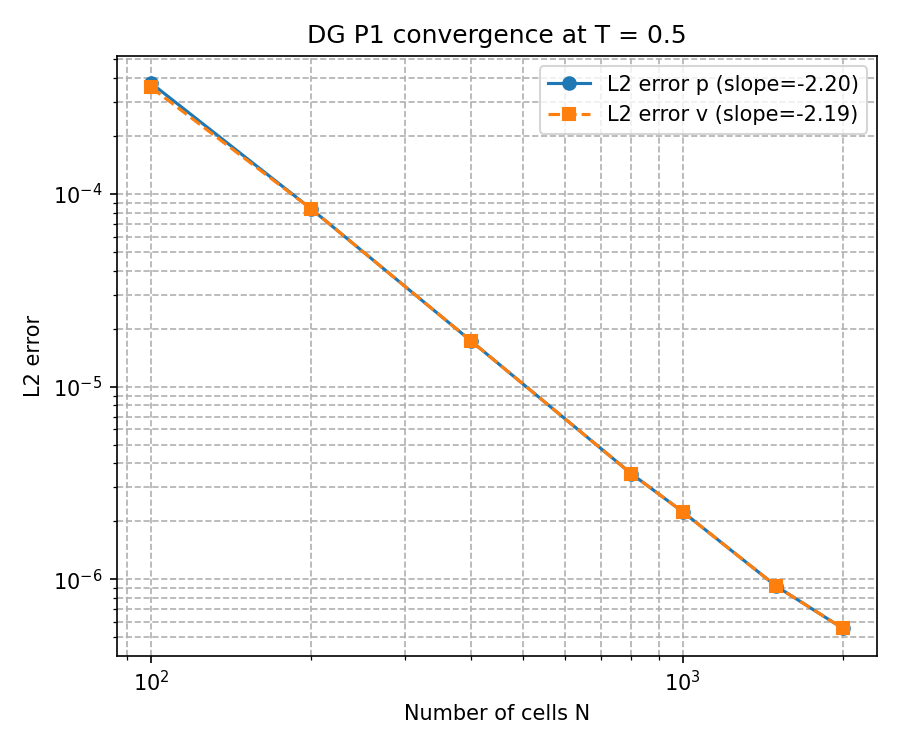
\includegraphics[width=\textwidth]{Images/dg_convergence_T0.5_rk2.png}
        \caption{Convergence of the DG method with RK2 scheme.}
        \label{fig:convergence_plot_rk2_t_05}
    \end{minipage}
\end{figure}

The numerical results confirm the theoretical convergence rates of the discontinuous Galerkin method.
For a polynomial degree $d$, the spatial discretization achieves an order of accuracy
$\mathcal{O}(h^{d+1})$ in the $L^2$ norm for sufficiently smooth solutions. \cite[Section~4.5]{HesthavenWarburton2008} 
The overall convergence rate of the fully discrete scheme is 
limited by the order of the time integration method: first order for 
the explicit Euler scheme and second order for the second-order 
Runge–Kutta scheme.

\begin{figure}[htbp]
    \centering
    \begin{minipage}[t]{0.48\textwidth}
        \centering
        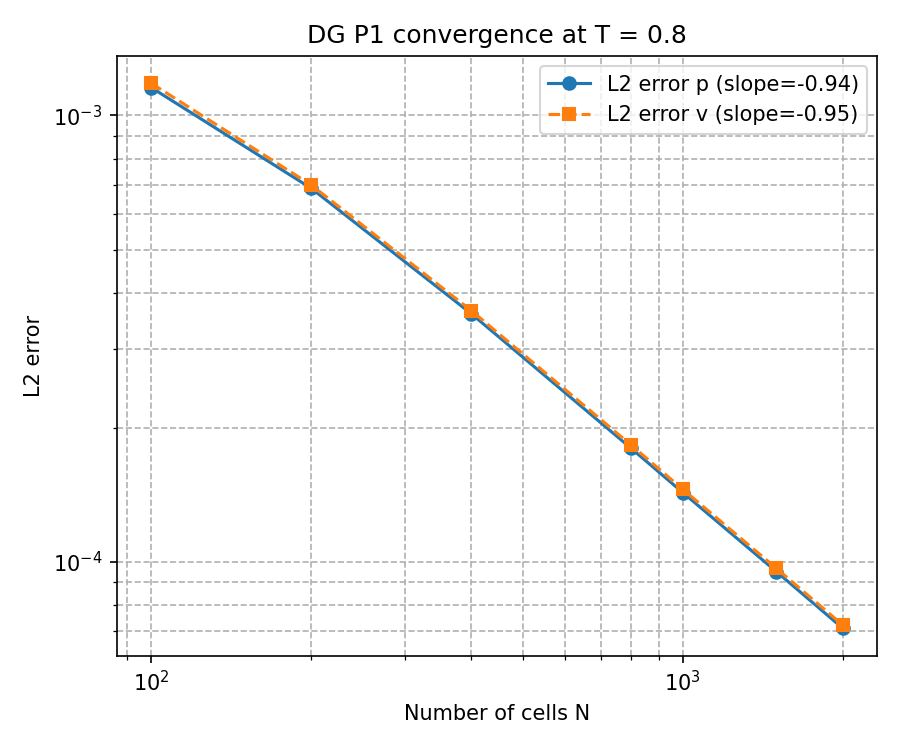
\includegraphics[width=\textwidth]{Images/dg_convergence_T0.8_euler.png}
        \caption{Convergence of the DG method with Explicit Euler scheme.}
        \label{fig:convergence_plot_euler_t_08}
    \end{minipage}
    \hfill
    \begin{minipage}[t]{0.48\textwidth}
        \centering
        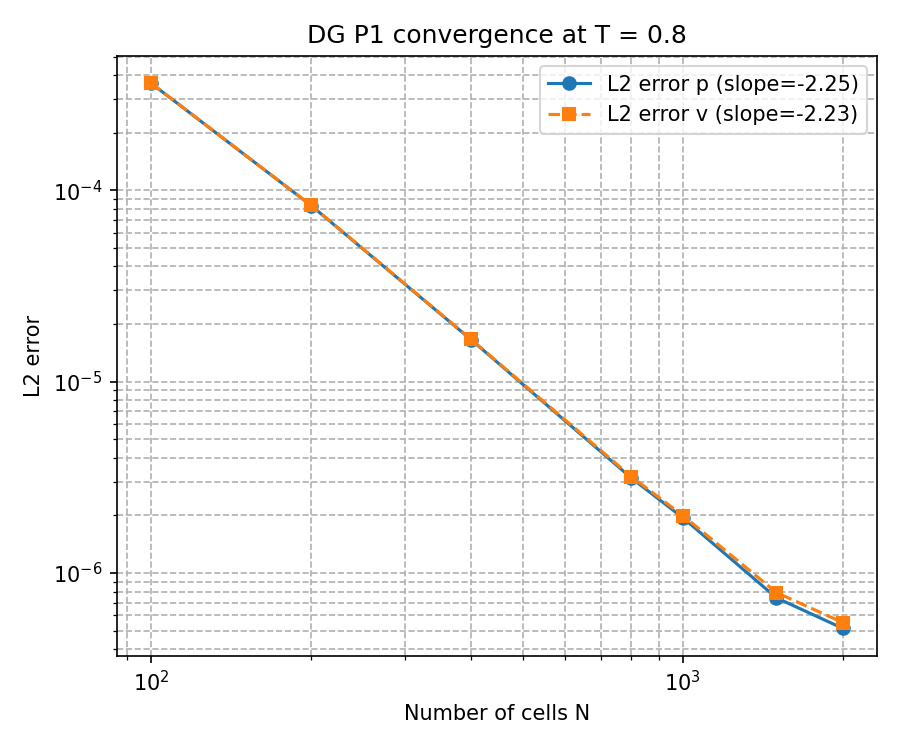
\includegraphics[width=\textwidth]{Images/dg_convergence_T0.8_rk2.png}
        \caption{Convergence of the DG method with Rk2 scheme.}
        \label{fig:convergence_plot_rk2_t_08}
    \end{minipage}
\end{figure}

As shown in Figures \ref{fig:convergence_plot_euler_t_08} and \ref{fig:convergence_plot_rk2_t_08},
the convergence behavior remains consistent even after the wave has interacted with the boundary.
This indicates that the boundary condition is correctly implemented (with similar order of accuracy for 
the DG solver and the Boundary condition solver) and so, does not affect the accuracy of the numerically
computed solution.

\subsection{Non-uniform cross-section}
In the case of a non-uniform cross-section $S(x) \neq S^*$, no analytical solution is available.
\subsubsection{Case of an exponential cross-section} $\\ \\$
We consider an exponential cross-section defined as
\begin{figure}[htbp]
    \centering
    \begin{minipage}[c]{0.4\textwidth}
        \centering
        \vfill
        \begin{equation}
            S(x) = S_0 \exp(k x)
        \end{equation}
        where $S_0 > 0$ and $k$ are given constants.
        \vfill
    \end{minipage}
    \hfill
    \begin{minipage}[c]{0.58\textwidth}
        \centering
        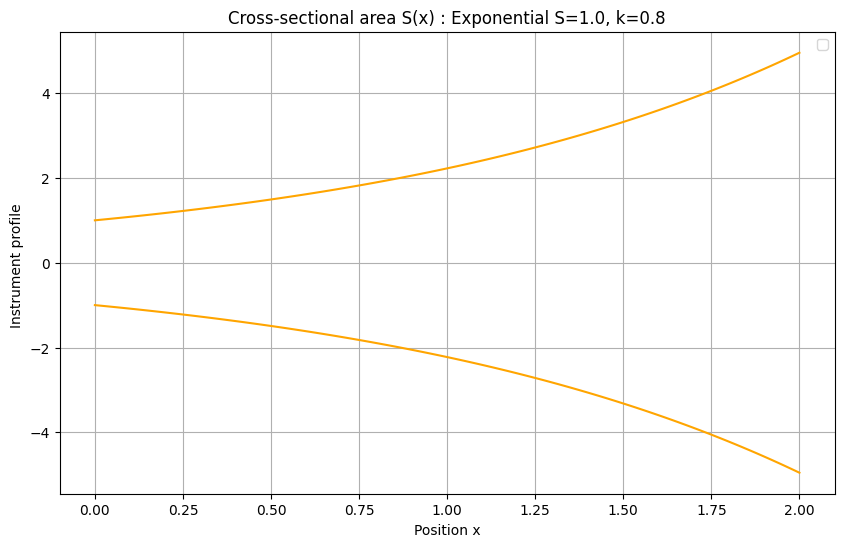
\includegraphics[width=0.8\textwidth]{Images/exp_profile.png}
    \end{minipage}
    \caption{Exponential variation of the cross-sectional area $S(x)$.}
    \label{fig:exp_profile}
\end{figure}

This is the shape of the clarinet bell for example.

\begin{figure}[htbp]
    \centering
    % Remplacez 'figs/dg_solution.png' par le chemin et l'extension réels de votre image (pdf, png, jpg...)
    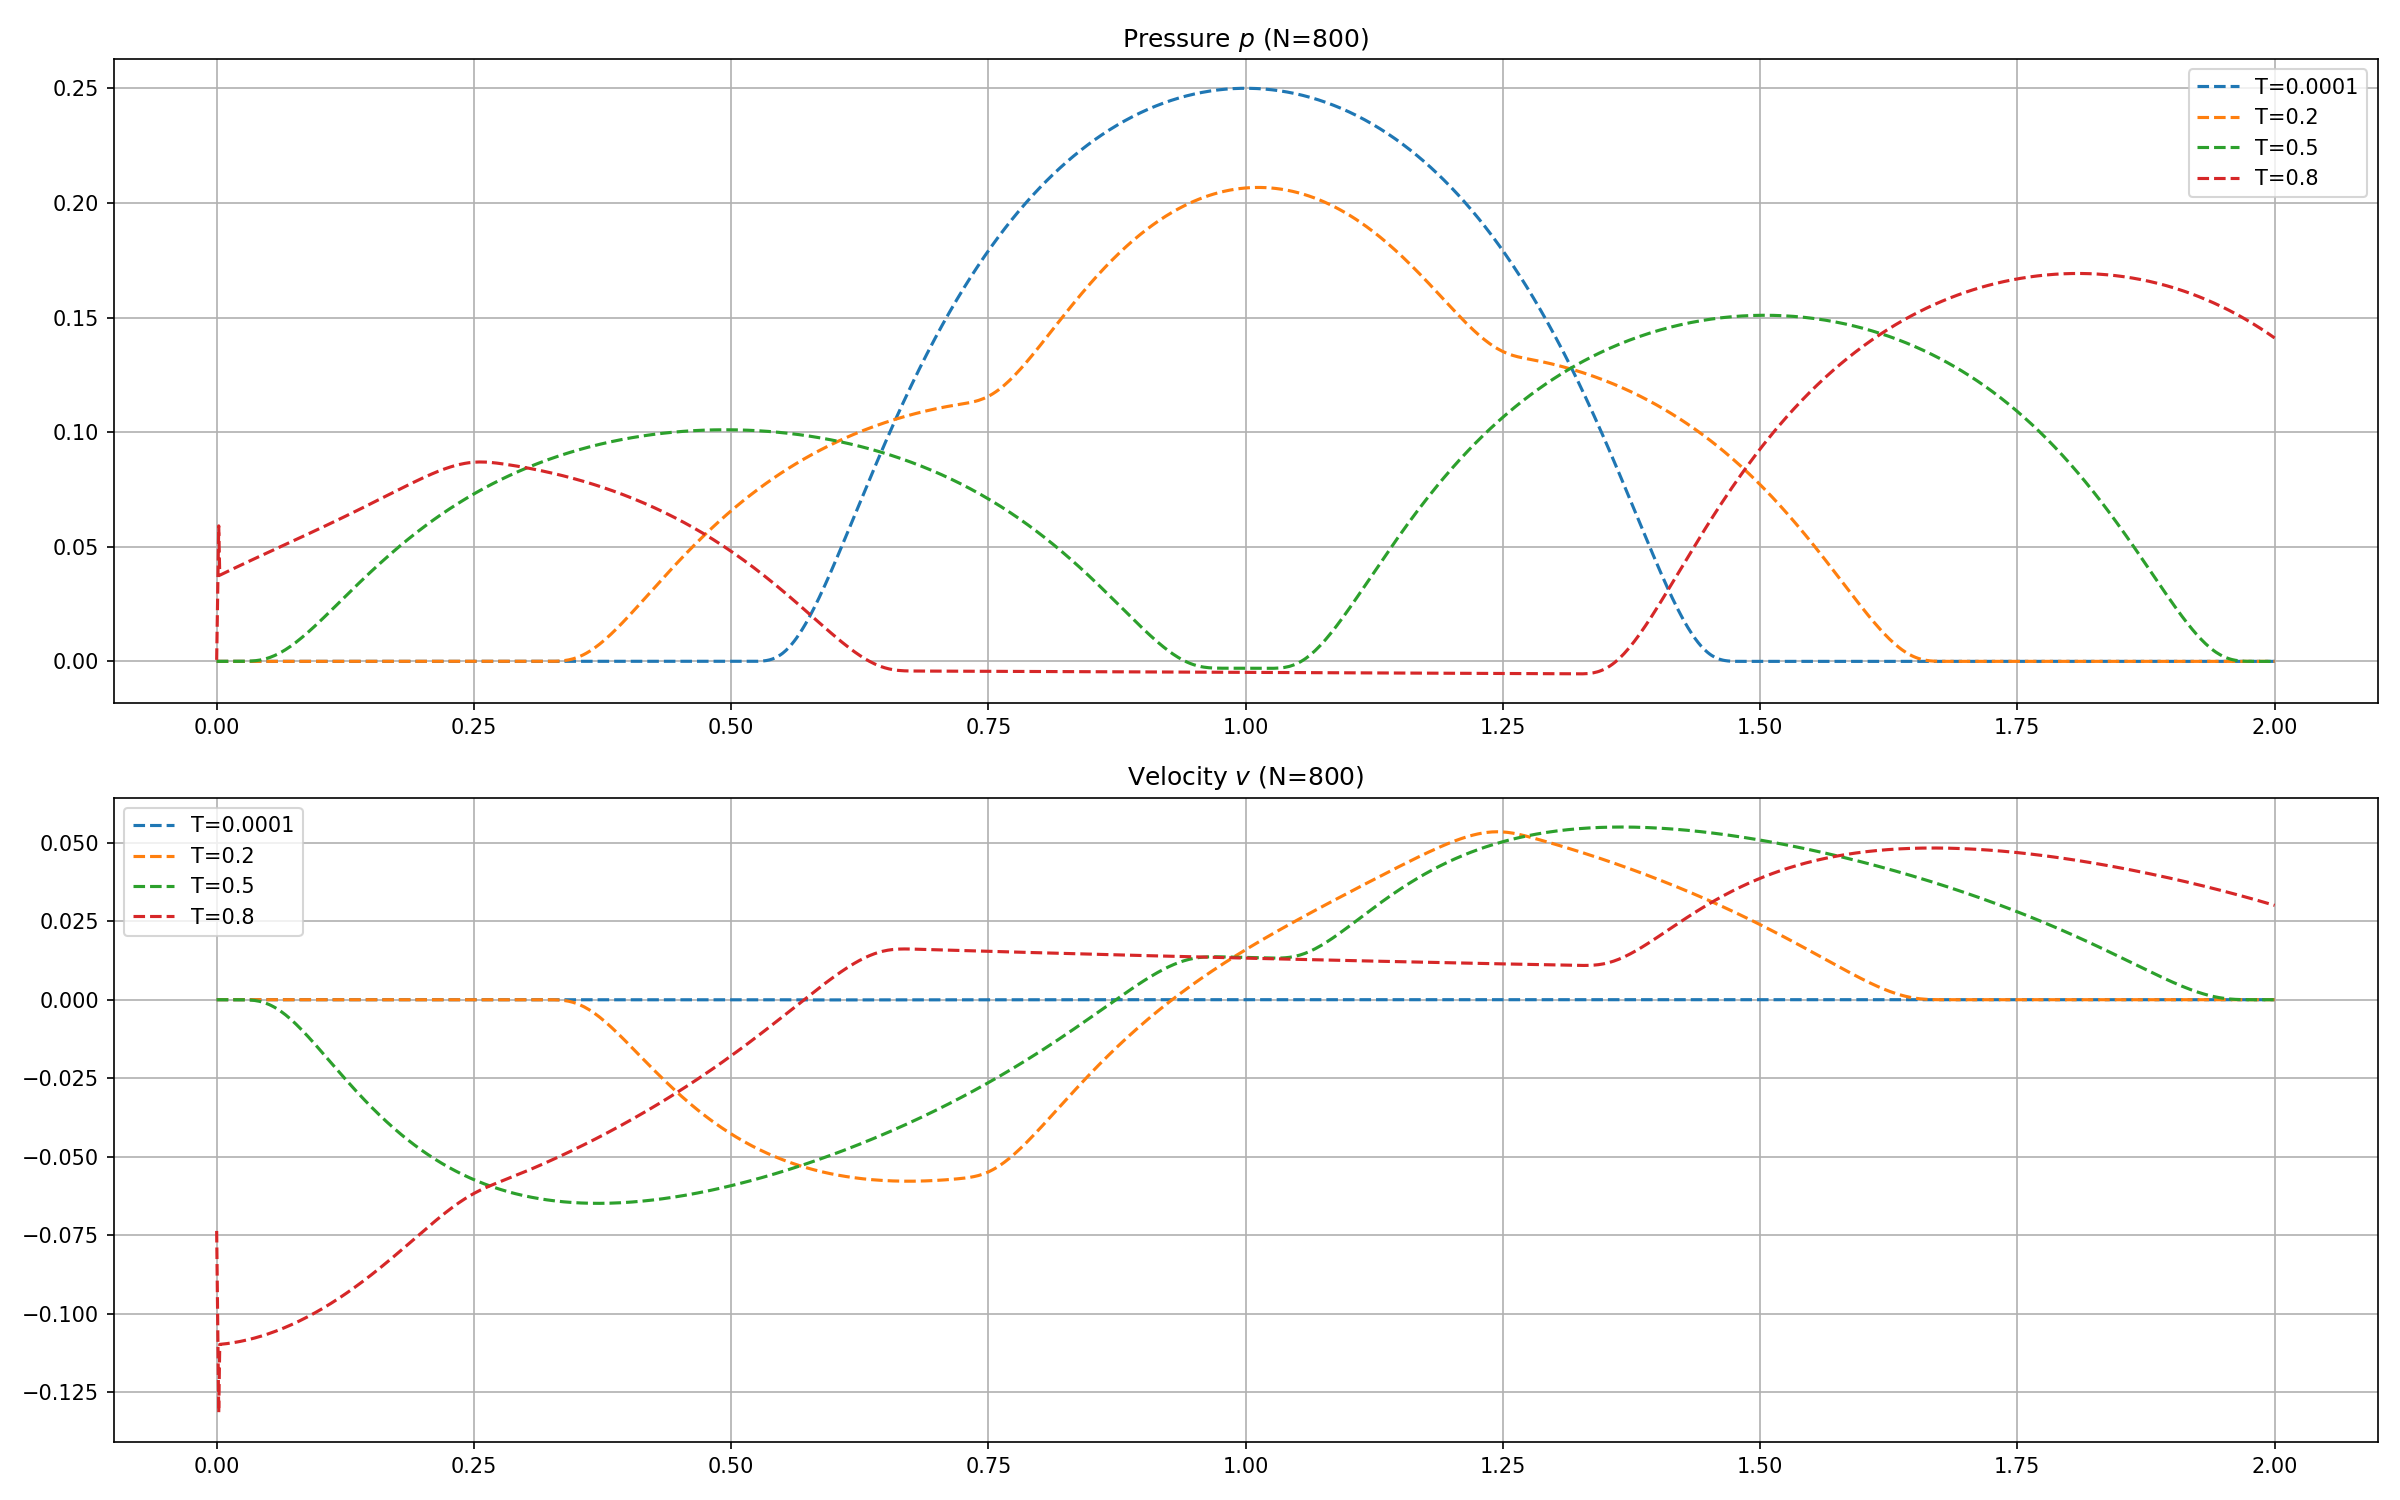
\includegraphics[width=0.9\textwidth]{Images/dg_solution_exp_N800.png}
    \caption{DG numerical solutions exponential cross-section.}
    \label{fig:dg_solution_exp}
\end{figure}

\newpage
\subsubsection{Case of a conical cross-section} $\\ \\$
We consider a conical cross-section defined as
\begin{figure}[htbp]
    \centering
    \begin{minipage}[c]{0.4\textwidth}
        \centering
        \vfill
        \begin{equation}
            S(x) = S_0 + k x
        \end{equation}
        where $S_0 > 0$ and $k$ are given constants.
        \vfill
    \end{minipage}
    \hfill
    \begin{minipage}[c]{0.58\textwidth}
        \centering
        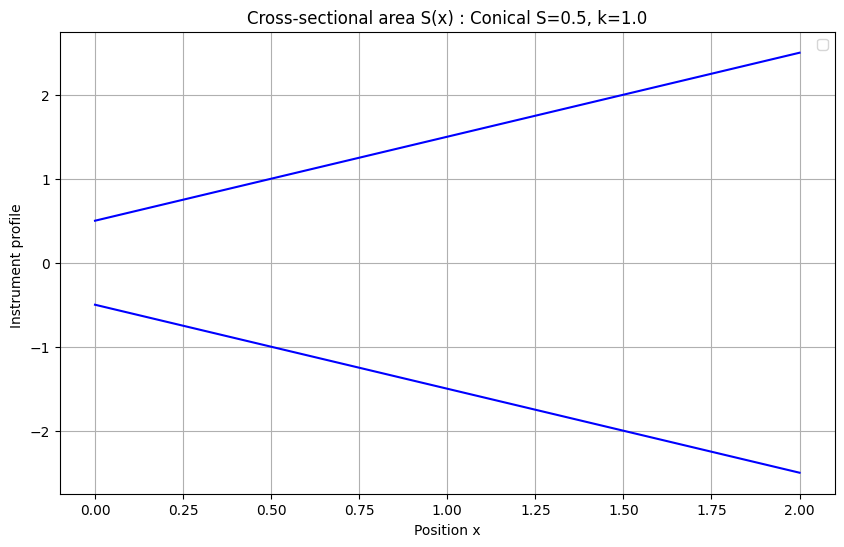
\includegraphics[width=0.8\textwidth]{Images/cone_profile.png}
    \end{minipage}
    \caption{Profile of an instrument with a conical cross-section.}
    \label{fig:cone_profile}
\end{figure}

This is another shape of musical instrument.
\newpage
\begin{figure}[htbp]
    \centering
    % Remplacez 'figs/dg_solution.png' par le chemin et l'extension réels de votre image (pdf, png, jpg...)
    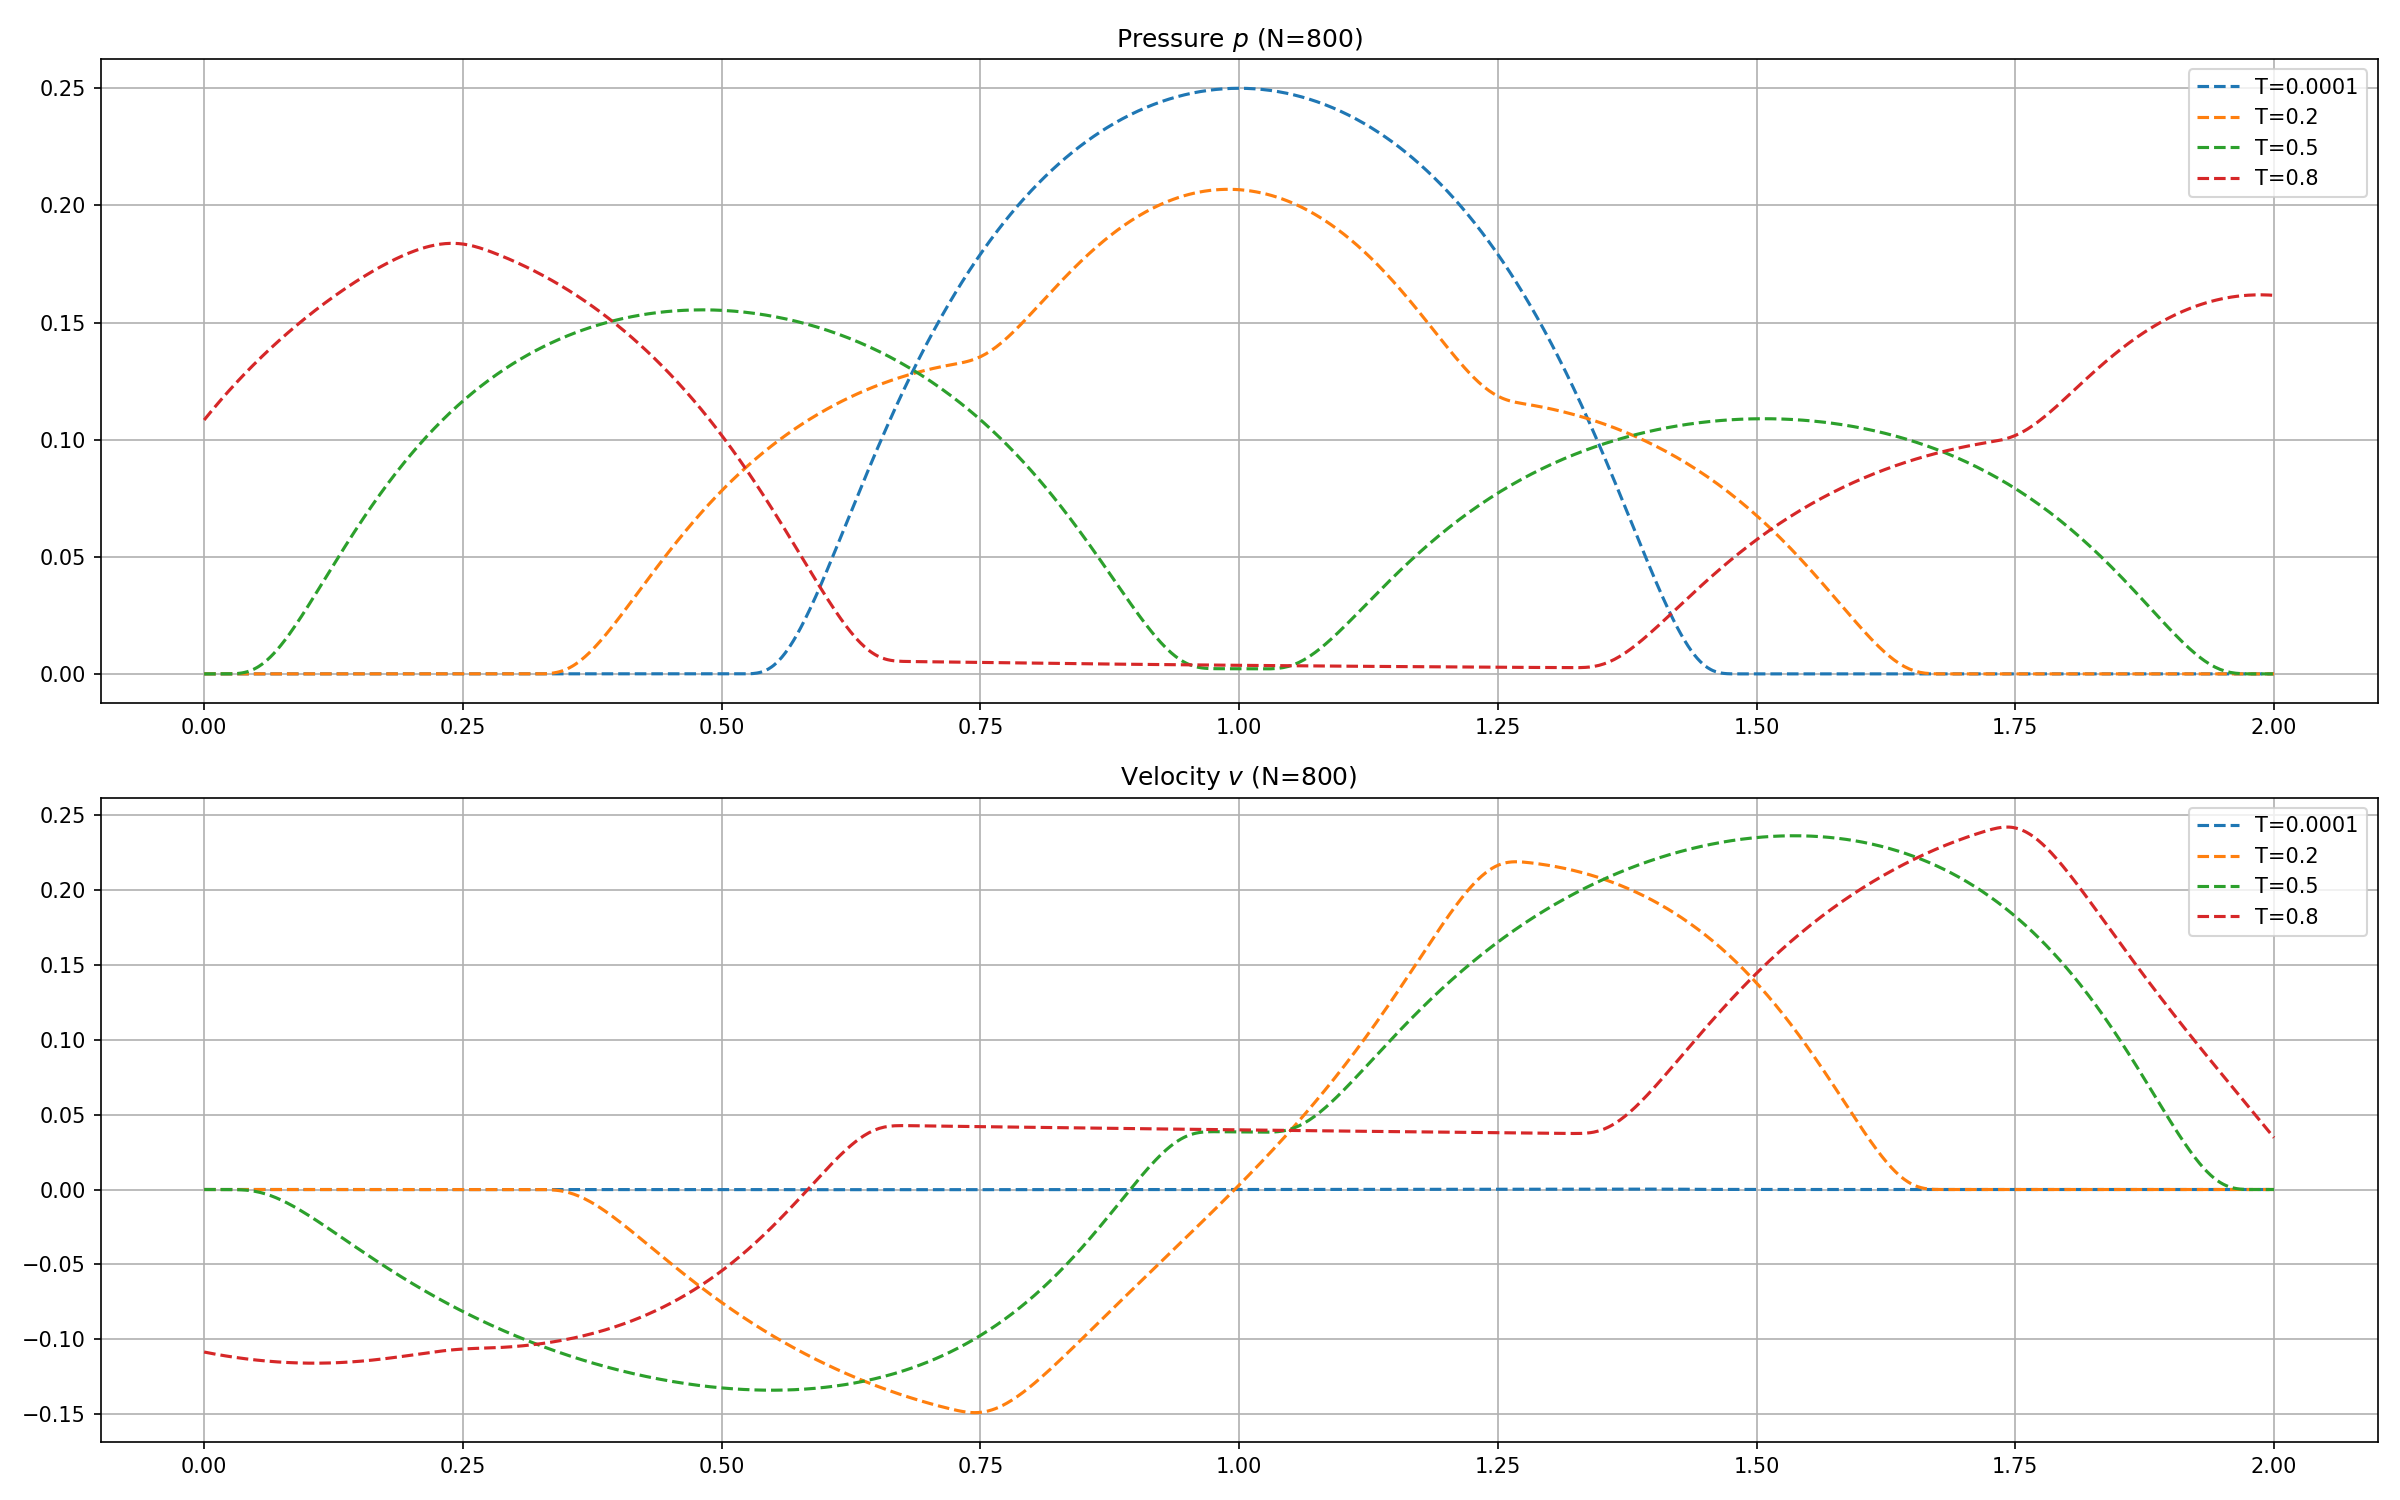
\includegraphics[width=0.9\textwidth]{Images/dg_solution_cone_N800.png}
    \caption{DG numerical solutions cone cross-section.}
    \label{fig:dg_solution_cone}
\end{figure}

The analysis of the numerical results for a non-uniform cross-section is more qualitative due 
to the absence of an analytical solution for direct comparison.
We can oberse that the wave propagation is influenced by the varying cross-sectional area,
as it has stop to be symmetric.
For example, the pressure is amplified in regions where the cross-sectional area decreases. 

Note: Since we assume the wave speed to be the maximum eigenvalue of $C^{-1}(x)A$, 
the Rusanov flux does not directly account for the variable cross-section. 
As the system is not strictly conservative, some numerical energy dissipation is observed 
(e.g., the pressure becomes negative in Figure~\ref{fig:dg_solution_exp}, 
and the acoustic velocity remains positive where it should vanish (see figures \ref{fig:dg_solution_exp} and \ref{fig:dg_solution_cone})).

\section{Performance Study}
A performance analysis was carried out to assess the computational efficiency of the Discontinuous Galerkin (DG) method implementation.
The study measured the execution time for simulations with different numbers of elements ($N$), using the parameters listed in 
Table~\ref{tab:sim_parameters}, with a final simulation time of $T = 0.5\ \mathrm{s}$.
\subsection{Euler explicit time integration}
\begin{table}[h!]
\centering
\begin{tabular}{c ccc}
\hline
$N \backslash S(x)$ & Const. & Exp. & Cone \\
\hline
100 & 0.250 & 0.154 & 0.142 \\
200 & 0.205 & 0.175 & 0.156 \\
300 & 0.238 & 0.213 & 0.198 \\
400 & 0.325 & 0.249 & 0.245 \\
500 & 0.344 & 0.326 & 0.296 \\
600 & 0.409 & 0.387 & 0.371 \\
700 & 0.569 & 0.545 & 0.522 \\
800 & 0.666 & 0.739 & 0.620 \\
1000 & 1.059 & 1.053 & 1.021 \\
1500 & 2.248 & 2.151 & 2.076 \\
2000 & 3.526 & 3.327 & 3.380 \\
\hline
\end{tabular}
\caption{Execution time (s) of the DG P1 solver using the EULER scheme.}
\label{tab:performance-euler}
\end{table}


\begin{figure}[htbp]
    \centering
    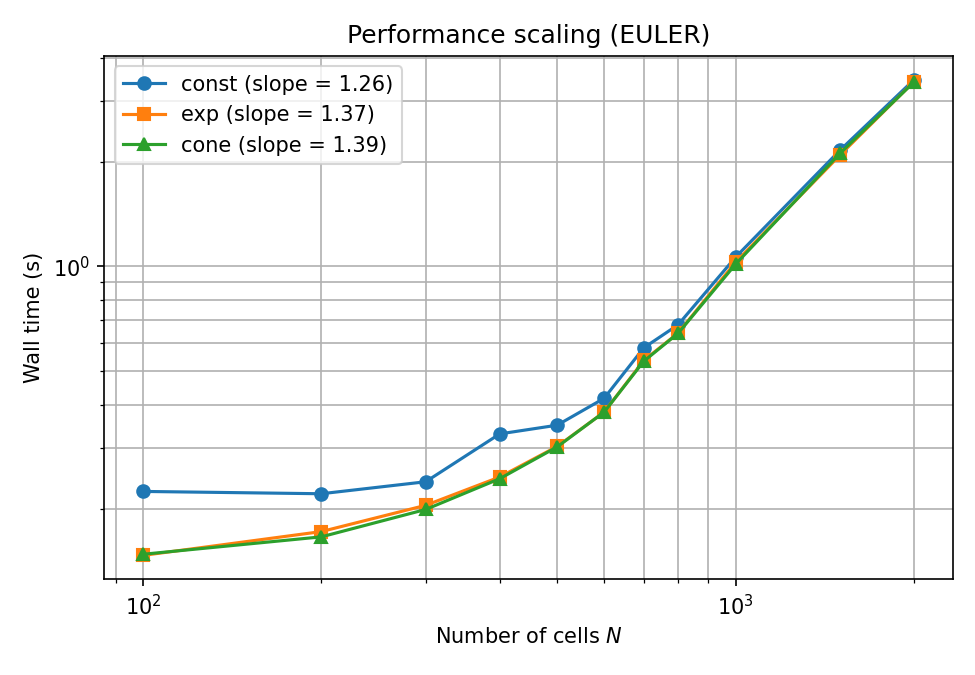
\includegraphics[width=0.7\textwidth]{Images/performance_euler.png}
    \caption{Performance study with Explicit Euler time integration.}
    \label{fig:performance_euler}
\end{figure}

The performance results indicate that the execution time scales under $N^2$. 
Since the performance study was done in JAX framework, the first run includes
compilation time. This explains the higher execution time for the smallest $N$ values 
for the constant cross-section case in Figure~\ref{fig:performance_euler}.

\newpage
\subsection{RK2 explicit time integration}

\begin{table}[h!]
\centering
\begin{tabular}{c ccc}
\hline
$N \backslash S(x)$ & Const. & Exp. & Cone \\
\hline
100 & 0.237 & 0.189 & 0.188 \\
200 & 0.325 & 0.218 & 0.225 \\
300 & 0.386 & 0.280 & 0.298 \\
400 & 0.503 & 0.386 & 0.376 \\
500 & 0.594 & 0.502 & 0.487 \\
600 & 0.720 & 0.639 & 0.624 \\
700 & 0.986 & 0.952 & 0.939 \\
800 & 1.205 & 1.162 & 1.173 \\
1000 & 2.079 & 1.943 & 1.962 \\
1500 & 3.931 & 4.024 & 3.937 \\
2000 & 6.579 & 6.484 & 6.693 \\
\hline
\end{tabular}
\caption{Execution time (s) of the DG P1 solver using the RK2 scheme.}
\label{tab:performance-rk2}
\end{table}

\newpage
\begin{figure}[htbp]
    \centering
    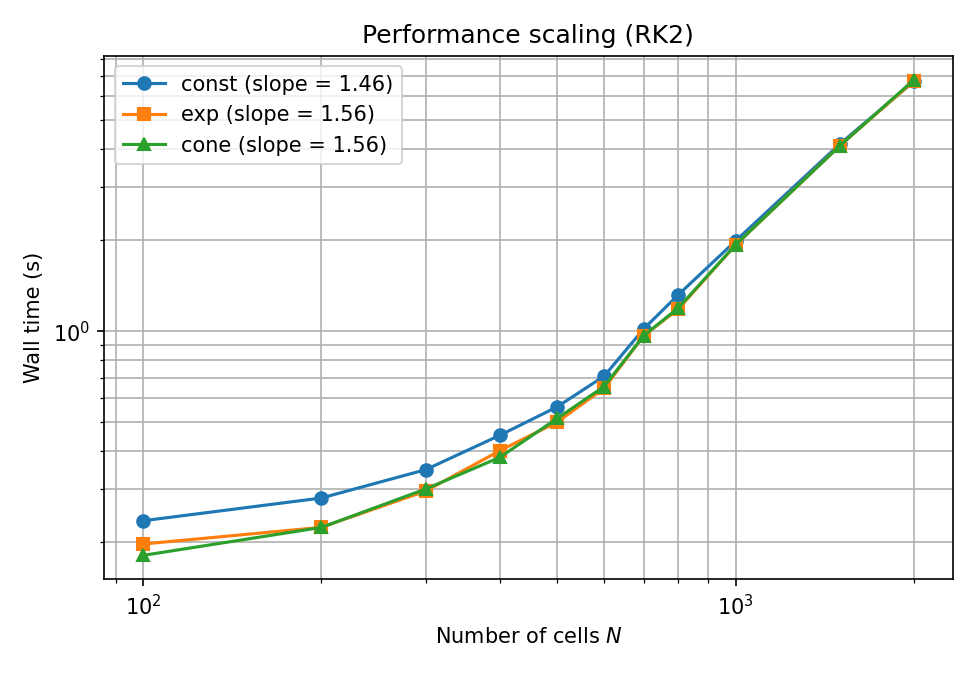
\includegraphics[width=0.7\textwidth]{Images/performance_rk2.png}
    \caption{Performance study with RK2 explicit time integration.}
    \label{fig:performance_rk2}
\end{figure}

The performance results for the RK2 explicit time integration scheme also show a scaling of execution time under $N^2$ 
but superior to the Euler explicit time integration scheme as expected due to the additional computations involved in the RK2 method.
That also explain the higher execution time in the performance study in Table~\ref{tab:performance-rk2}.
 
\newpage
\chapter{Conclusion}
The main objective of my third-semester Master’s project was to develop a framework for the automated calibration of a set of parameters 
governing wave propagation inside a reed instrument. To achieve this goal, I implemented a Discontinuous Galerkin Method (DGM) solver for 
the one-dimensional mixed formulation of the acoustic wave equation in a duct with variable cross-sectional area.

The primary challenges of this work were the correct formulation of the DGM for the mixed wave system, the implementation of the radiation 
boundary condition at the open end of the instrument, and the validation of the numerical solver against an analytical solution in the 
simplified case of a constant cross-sectional area. Particular attention was paid to the consistent treatment of boundary conditions, which 
play a crucial role in accurately modeling wave reflection and radiation phenomena in wind instruments.

The solver was implemented using the JAX framework, enabling just-in-time compilation and paving the way for future developments involving 
automatic differentiation. Both Explicit Euler and second-order Runge–Kutta (RK2) time integration schemes were implemented and tested. 
Numerical experiments demonstrated that the proposed DGM solver is accurate and stable for wave propagation in ducts with both uniform and 
non-uniform cross-sectional profiles. Furthermore, a convergence study confirmed that the numerical method achieves the expected theoretical 
rates of convergence. Performance analyses showed that the JAX-based implementation scales efficiently with the number of elements, making 
it suitable for large-scale simulations required in calibration and optimization tasks.

Future work will focus on extending the solver to handle a fully conservative system of equations, 
as well as implementing the complete right-hand-side boundary conditions described by 
equations~\eqref{eq:1e} and~\eqref{eq:1f}, which are essential for accurately modeling the 
reed–instrument interaction. Additionally, further investigations will be required to develop 
an effective automated calibration strategy, including data preprocessing, parameter selection, 
and the choice of appropriate loss functions for optimization.

I would like to express my sincere gratitude to my supervisors—Dr. Emmanuel Franck, Dr. Juliette Chabassier, Dr. Laurent Navoret, Dr. Victor
 Michel-Dansac, and Dr. Alexis Thibault—for their invaluable guidance, insightful discussions, and continuous support throughout this project.

\newpage
\printbibliography

% Minimal example of an external bibliography (create refs.bib)
% Example BibTeX entry:
%
% @article{doe2020,
%   author = {Doe, John and Example, Anne},
%   title = {Title of the cited article},
%   journal = {Example Journal},
%   year = {2020},
%   volume = {12},
%   pages = {34--56}
% }

\end{document}